% answers.tex —— 2010 年·普通高等学校招生考试·陕西卷·文科 · 参考答案与详细解析片段
% 由 tools/generate_projects.py 依来源总账自 2010/2010_数学真题_陕西文_试题.md + 2010/2010_数学真题_陕西文_解析正文.md + 2010/2010_数学真题_陕西文_答案要点.md 生成，勿手改（改源 MD 后重跑）
\begin{gktip}
固定候选 PDF 仅含题面、无答案页；以下解析与结论均由本库独立推导（非官方答案），并按 600 dpi 原页逐题复核题面。原页未印分值，不补。

【源疑点】原页第 5 题四个选项排在同一行，(A) 与 (B) 之间没有留间距，(A) 的右括号与「(B)」紧贴，属排版挤压而非选项内容有误；题面照录，两个选项的内容分别按 $S=S*(n+1)$ 与 $S=S*x_{n+1}$ 读。

【源疑点】原页第 10 题印作「某学校要招开学生代表大会」，「招开」疑为「召开」之误印；题面照录不改，不影响作答。

【源疑点】原页第 15 题为「15．三选一．」，下分【A】【B】【C】三小题，未印「选考题」栏目名，也未印「考生只能从 A、B、C 三题中任选一题作答」的说明；按课标卷体例这三小题分属不等式选讲、几何证明选讲、坐标系与参数方程，属选修模块选考。此处照录，不改栏目名。
\end{gktip}

\begin{answer}
\gksolhead{1}{}

\textbf{题目}：

集合 $A=\{x\mid -1\leqslant x\leqslant 2\}$，$B=\{x\mid x<1\}$，则 $A\cap B=$（　）

（A）$\{x\mid x<1\}$

（B）$\{x\mid -1\leqslant x\leqslant 2\}$

（C）$\{x\mid -1\leqslant x\leqslant 1\}$

（D）$\{x\mid -1\leqslant x<1\}$

\Needspace{4\baselineskip}
\textbf{解析}

\Needspace{5\baselineskip}
$A=\{x\mid -1\leqslant x\leqslant 2\}$，$B=\{x\mid x<1\}$。交集是同时属于两个集合的元素，即同时满足
\nopagebreak[4]
\[-1\leqslant x\leqslant 2\quad\text{\text{与}}\quad x<1.\]
\Needspace{5\baselineskip}
把 $x<1$ 与 $x\geqslant -1$ 合并，得
\nopagebreak[4]
\[A\cap B=\{x\mid -1\leqslant x<1\}.\]
逐项核对：A 中 $\{x\mid x<1\}$ 含 $x<-1$ 的部分，超出 $A$；B 中 $\{x\mid -1\leqslant x\leqslant 2\}$ 就是 $A$ 本身，多出 $x\geqslant 1$ 的一段；C 中 $x\leqslant 1$ 把端点 $x=1$ 也收进来，而 $1\notin B$；只有 D 与计算结果一致。
端点代回检验：$x=-1$ 时 $-1\in A$ 且 $-1<1$，故 $-1$ 应属于交集，A、C 都漏掉它；$x=1$ 时 $1\in A$ 但 $1\notin B$，故 $1$ 不属于交集，C 多出它。
故选 D。

\gkanswer{答案：D。}

\end{answer}
\begin{answer}
\gksolhead{2}{}

\textbf{题目}：

复数 $z=\dfrac{\mathrm i}{1+\mathrm i}$ 在复平面上对应的点位于（　）

（A）第一象限

（B）第二象限

（C）第三象限

（D）第四象限

\Needspace{4\baselineskip}
\textbf{解析}

\Needspace{5\baselineskip}
分母实数化：
\nopagebreak[4]
\[z=\frac{\mathrm i}{1+\mathrm i}=\frac{\mathrm i(1-\mathrm i)}{(1+\mathrm i)(1-\mathrm i)}=\frac{\mathrm i-\mathrm i^2}{1^2+1^2}=\frac{1+\mathrm i}{2}=\frac12+\frac12\mathrm i.\]
实部 $\dfrac12>0$，虚部 $\dfrac12>0$，对应点为 $\left(\dfrac12,\dfrac12\right)$，位于第一象限。
逐项核对：第二象限需实部为负、虚部为正；第三象限需实部、虚部均为负；第四象限需实部为正、虚部为负。均不符。
故选 A。

\gkanswer{答案：A。}

\end{answer}
\begin{answer}
\gksolhead{3}{}

\textbf{题目}：

函数 $f(x)=2\sin x\cos x$ 是（　）

（A）最小正周期为 $2\pi$ 的奇函数

（B）最小正周期为 $2\pi$ 的偶函数

（C）最小正周期为 $\pi$ 的奇函数

（D）最小正周期为 $\pi$ 的偶函数

\Needspace{4\baselineskip}
\textbf{解析}

\Needspace{5\baselineskip}
先用二倍角公式化简：
\nopagebreak[4]
\[f(x)=2\sin x\cos x=\sin 2x.\]
（A）（B）最小正周期 $T=\dfrac{2\pi}{2}=\pi$，故两项的周期 $2\pi$ 均错。
（C）（D）$\sin(-2x)=-\sin 2x$，即 $f(-x)=-f(x)$，$f$ 为奇函数，故 C 对、D 错。
故选 C。

\gkanswer{答案：C。}

\end{answer}
\begin{answer}
\gksolhead{4}{}

\textbf{题目}：

如图，样本 $A$ 和 $B$ 分别取自两个不同的总体，它们的样本平均数分别为 $\bar x_A$ 和 $\bar x_B$，样本标准差分别为 $s_A$ 和 $s_B$，则（　）

（A）$\bar x_A>\bar x_B$，$s_A>s_B$

（B）$\bar x_A<\bar x_B$，$s_A>s_B$

（C）$\bar x_A>\bar x_B$，$s_A<s_B$

（D）$\bar x_A<\bar x_B$，$s_A<s_B$
\nopagebreak[4]
\begin{center}% 2010 年陕西卷文科第 4 题：样本 A、B 的折线图（纵轴为样本值，横轴为 n）。
% 来源 PDF：普通高考/2010/2010陕西文.pdf，SHA-256 428bcb4aee4c6a7a6a9c9d0dca1377b14112594015d1d50a931e725ae0c5c130。
% 原页：第 1 页（A3 三栏）第 1 栏中部，书页码 625。
% 重绘依据：照原页——左图标题 A、右图标题 B；两图均为方格纸，纵轴标 5、10、15，
%   横轴标 0、2、4、6 并在末端加箭头标 n；方格为正方形，横轴每 1 个单位一格，
%   纵轴每 2.5 个单位一格（故 5、10、15 隔一格标注一次），方格框右、上各多出一格。
%   按原页读点（横轴 n=1,…,6）：图 A 依次为 2.5、10、5、7.5、2.5、10；
%   图 B 依次为 15、10、12.5、10、12.5、10。
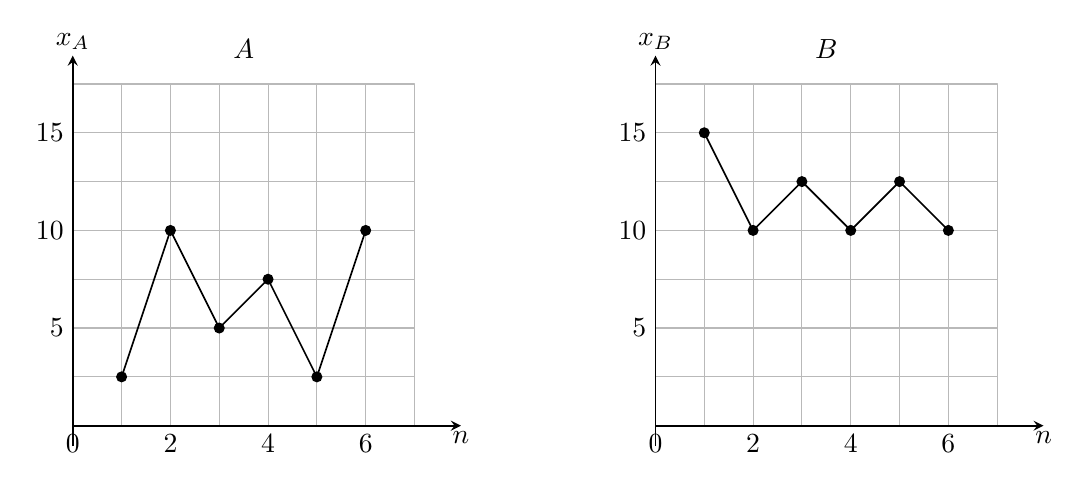
\begin{tikzpicture}[semithick, x=0.62cm, y=0.248cm, line join=round,
  gridl/.style={thin, gray!55}]

  % ================= 图 A =================
  \begin{scope}
    \draw[gridl] (0,0) rectangle (7,17.5);
    \foreach \i in {1,2,3,4,5,6} { \draw[gridl] (\i,0) -- (\i,17.5); }
    \foreach \j in {2.5,5,7.5,10,12.5,15} { \draw[gridl] (0,\j) -- (7,\j); }

    \draw[->, >=stealth] (0,-1.05) -- (0,18.95) node[above, inner sep=2pt] {$x_A$};
    \draw[->, >=stealth] (0,0) -- (7.95,0) node[below, inner sep=2pt] {$n$};

    \foreach \i/\v in {0/0, 2/2, 4/4, 6/6} {
      \node[below, inner sep=3pt] at (\i,0) {$\v$};
    }
    \foreach \j/\v in {5/5, 10/10, 15/15} {
      \node[left, inner sep=3pt] at (0,\j) {$\v$};
    }
    \node at (3.5,19.3) {$A$};

    \draw (1,2.5) -- (2,10) -- (3,5) -- (4,7.5) -- (5,2.5) -- (6,10);
    \foreach \p in {(1,2.5), (2,10), (3,5), (4,7.5), (5,2.5), (6,10)} {
      \fill \p circle (2.0pt);
    }
  \end{scope}

  % ================= 图 B =================
  \begin{scope}[xshift=7.40cm]
    \draw[gridl] (0,0) rectangle (7,17.5);
    \foreach \i in {1,2,3,4,5,6} { \draw[gridl] (\i,0) -- (\i,17.5); }
    \foreach \j in {2.5,5,7.5,10,12.5,15} { \draw[gridl] (0,\j) -- (7,\j); }

    \draw[->, >=stealth] (0,-1.05) -- (0,18.95) node[above, inner sep=2pt] {$x_B$};
    \draw[->, >=stealth] (0,0) -- (7.95,0) node[below, inner sep=2pt] {$n$};

    \foreach \i/\v in {0/0, 2/2, 4/4, 6/6} {
      \node[below, inner sep=3pt] at (\i,0) {$\v$};
    }
    \foreach \j/\v in {5/5, 10/10, 15/15} {
      \node[left, inner sep=3pt] at (0,\j) {$\v$};
    }
    \node at (3.5,19.3) {$B$};

    \draw (1,15) -- (2,10) -- (3,12.5) -- (4,10) -- (5,12.5) -- (6,10);
    \foreach \p in {(1,15), (2,10), (3,12.5), (4,10), (5,12.5), (6,10)} {
      \fill \p circle (2.0pt);
    }
  \end{scope}
\end{tikzpicture}
\end{center}
\nopagebreak[4]
\Needspace{4\baselineskip}
\textbf{解析}

【图注】原页并排两幅方格折线图，左图标题 $A$、右图标题 $B$；纵轴标 $x_A$、$x_B$，刻度 $5$、$10$、$15$，横轴标 $n$，刻度 $0$、$2$、$4$、$6$。方格为正方形：横轴每 $1$ 个单位一格，纵轴每 $2.5$ 个单位一格，故纵轴刻度隔一格标注一次。两图最上、最右各多画一格，是方格纸的边界，不是数据点。

\Needspace{5\baselineskip}
按格点读出六个样本值（$n=1,2,\dots,6$）：
\nopagebreak[4]
\[A:\ 2.5,\ 10,\ 5,\ 7.5,\ 2.5,\ 10;\qquad B:\ 15,\ 10,\ 12.5,\ 10,\ 12.5,\ 10.\]
\Needspace{5\baselineskip}
求平均数：
\nopagebreak[4]
\[\bar x_A=\frac{2.5+10+5+7.5+2.5+10}{6}=\frac{37.5}{6}=6.25,\]
\nopagebreak[4]
\[\bar x_B=\frac{15+10+12.5+10+12.5+10}{6}=\frac{70}{6}\approx 11.67,\]
故 $\bar x_A<\bar x_B$。

\Needspace{5\baselineskip}
再比离散程度。$A$ 的取值在 $2.5$ 与 $10$ 之间大起大落，与 $\bar x_A$ 的偏差分别为 $-3.75$、$3.75$、$-1.25$、$1.25$、$-3.75$、$3.75$，平方和
\nopagebreak[4]
\[\sum_{i=1}^{6}(x_i-\bar x_A)^2=4\times 3.75^2+2\times 1.25^2=56.25+3.125=59.375.\]
\Needspace{5\baselineskip}
$B$ 的取值只在 $10$ 与 $15$ 之间小幅往返，偏差最大约 $3.33$，平方和
\nopagebreak[4]
\[\sum_{i=1}^{6}(x_i-\bar x_B)^2=\frac{100}{9}+3\cdot\frac{25}{9}+2\cdot\frac{25}{36}=\frac{375}{18}\approx 20.83,\]
明显小于 $59.375$。样本标准差 $s=\sqrt{\dfrac1n\sum(x_i-\bar x)^2}$ 与平方和同序，故 $s_A>s_B$。
合起来：$\bar x_A<\bar x_B$ 且 $s_A>s_B$。逐项核对：A、C 把平均数大小弄反；D 把标准差大小弄反。
故选 B。

\gkanswer{答案：B。}

\end{answer}
\begin{answer}
\gksolhead{5}{}

\textbf{题目}：

如图是求 $x_1$，$x_2$，$\cdots$，$x_{10}$ 的乘积 $S$ 的程序框图，图中空白框中应填入的内容为（　）

（A）$S=S*(n+1)$

（B）$S=S*x_{n+1}$

（C）$S=S*n$

（D）$S=S*x_n$
\nopagebreak[4]
\begin{center}% 2010 年陕西卷文科第 5 题：求 x1,x2,…,x10 的乘积 S 的程序框图。
% 来源 PDF：普通高考/2010/2010陕西文.pdf，SHA-256 428bcb4aee4c6a7a6a9c9d0dca1377b14112594015d1d50a931e725ae0c5c130。
% 原页：第 1 页（A3 三栏）第 1 栏下部，书页码 625。
% 重绘依据：照原页——竖排主干为 开始→输入 x1,…,x10→n=1,S=1→〔空白框〕→判断 n≥10?
%   →「是」向下进 输出 S→结束；「否」向左进 n=n+1 框，该框顶部再向上折回主干，
%   在空白框正上方汇入主干（原页此处只在空白框上方画一个向下箭头）。空白框在原页为空。
\begin{tikzpicture}[semithick,
  every node/.style={inner sep=2pt},
  box/.style={draw, minimum width=3.6cm, minimum height=0.66cm, align=center},
  round/.style={draw, rounded corners=7pt, minimum width=1.7cm,
    minimum height=0.66cm, align=center},
  para/.style={draw, trapezium, trapezium left angle=72, trapezium right angle=108,
    minimum width=6.2cm, minimum height=0.74cm, align=center},
  paraout/.style={draw, trapezium, trapezium left angle=72, trapezium right angle=108,
    minimum width=3.0cm, minimum height=0.74cm, align=center},
  dec/.style={draw, diamond, aspect=2.7, minimum width=2.9cm,
    minimum height=1.05cm, align=center},
  arr/.style={->, >=stealth}]

  \node[round] (start) at (0,0) {开始};
  \node[para]  (in)    at (0,-1.20) {输入 $x_1,\,x_2,\,\cdots,\,x_{10}$};
  \node[box]   (init)  at (0,-2.45) {$n=1$，$S=1$};
  \node[box, minimum height=0.86cm] (acc) at (0,-3.80) {};
  \node[dec]   (test)  at (0,-5.60) {$n\geqslant 10$};
  \node[box]   (inc)   at (-4.55,-3.80) {$n=n+1$};
  \node[paraout] (out)  at (0,-7.15) {输出 $S$};
  \node[round] (end)   at (0,-8.70) {结束};

  \draw[arr] (start) -- (in);
  \draw[arr] (in) -- (init);
  \draw[arr] (init) -- (acc);
  \draw[arr] (acc) -- (test);

  \draw[arr] (test) -- (out);
  \node[right] at (0.16,-6.40) {是};
  \draw[arr] (out) -- (end);

  % 「否」分支：由判断框左顶点向左，再向上进入 n=n+1 框
  \draw[arr] (test.west) -- (-4.55,-5.60) -- (inc.south);
  \node[above] at (-2.55,-5.45) {否};

  % 回边：n=n+1 框顶部向上、再向右，汇入空白框上方的竖线
  \draw (inc.north) -- (-4.55,-2.95) -- (0,-2.95);
\end{tikzpicture}
\end{center}
\nopagebreak[4]
\Needspace{4\baselineskip}
\textbf{解析}

按框图逐步追踪。赋初值 $n=1$，$S=1$ 后，每轮顺序为：先执行空白框，再判断 $n\geqslant 10$——不成立就执行 $n=n+1$ 并回到空白框，成立就输出 $S$。

\Needspace{5\baselineskip}
最终输出的 $S$ 必须是 $x_1x_2\cdots x_{10}$，而 $S$ 初值为 $1$（乘法的单位元），所以空白框只能是把当前项乘进 $S$：
\nopagebreak[4]
\[S=S*x_n.\]
第 $1$ 轮 $S=1\cdot x_1$，第 $2$ 轮 $S=x_1x_2$，……第 $10$ 轮 $S=x_1x_2\cdots x_{10}$，此时 $n=10$ 使判断成立而退出循环，恰好十项全部乘完。

逐项核对：A 每轮乘 $n+1$，十轮后 $S=2\times 3\times\cdots\times 11$，与数据无关；B 每轮乘 $x_{n+1}$，十轮后 $S=x_2x_3\cdots x_{11}$，首项 $x_1$ 漏乘、末项多乘了不存在的 $x_{11}$；C 每轮乘 $n$，十轮后 $S=10!$，同样与数据无关。
故选 D。

\gkanswer{答案：D。}

\end{answer}
\begin{answer}
\gksolhead{6}{}

\textbf{题目}：

“$a>0$”是“$|a|>0$”的（　）

（A）充分不必要条件

（B）必要不充分条件

（C）充要条件

（D）既不充分也不必要条件

\Needspace{4\baselineskip}
\textbf{解析}

命题 $p$：$a>0$；命题 $q$：$|a|>0$ 即 $a\neq 0$。
充分性：若 $a>0$，则 $|a|=a>0$，$p\Rightarrow q$ 成立。
必要性：取 $a=-1$，则 $|a|=1>0$，$q$ 成立但 $a>0$ 不成立，故 $q\not\Rightarrow p$。
所以 $p$ 是 $q$ 的充分不必要条件。逐项核对：B 把充分、必要弄反；C 忽视了负数反例；D 否定了已经成立的充分性。
故选 A。

\gkanswer{答案：A。}

\end{answer}
\begin{answer}
\gksolhead{7}{}

\textbf{题目}：

下列四类函数中，具有性质“对任意的 $x>0$，$y>0$，函数 $f(x)$ 满足 $f(x+y)=f(x)f(y)$”的是（　）

（A）幂函数

（B）对数函数

（C）指数函数

（D）余弦函数

\Needspace{4\baselineskip}
\textbf{解析}

把 $f(x+y)=f(x)f(y)$ 逐类检验。
（A）幂函数 $f(x)=x^\alpha$：$(x+y)^\alpha$ 一般不等于 $x^\alpha y^\alpha$。取 $\alpha=2$、$x=y=1$：左边 $4$，右边 $1$，不符。
（B）对数函数 $f(x)=\log_a x$：取 $x=y=1$，左边 $f(2)=\log_a 2\neq 0$，右边 $f(1)f(1)=0\cdot 0=0$，不符。
（C）指数函数 $f(x)=a^x$（$a>0$，$a\neq1$）：$f(x+y)=a^{x+y}=a^x\cdot a^y=f(x)f(y)$，对任意 $x>0$、$y>0$ 成立，符合。
（D）余弦函数 $f(x)=\cos x$：$\cos(x+y)=\cos x\cos y-\sin x\sin y$，多出一项 $-\sin x\sin y$。取 $x=y=\dfrac\pi4$：左边 $\cos\dfrac\pi2=0$，右边 $\dfrac12$，不符。
故选 C。

\gkanswer{答案：C。}

\end{answer}
\begin{answer}
\gksolhead{8}{}

\textbf{题目}：

若某空间几何体的三视图如图所示，则该几何体的体积是（　）

（A）$2$

（B）$1$

（C）$\dfrac23$

（D）$\dfrac13$
\nopagebreak[4]
\begin{center}% 2010 年陕西卷文科第 8 题：某空间几何体的三视图。
% 来源 PDF：普通高考/2010/2010陕西文.pdf，SHA-256 428bcb4aee4c6a7a6a9c9d0dca1377b14112594015d1d50a931e725ae0c5c130。
% 原页：第 1 页（A3 三栏）第 2 栏中部，书页码 625。
% 重绘依据：照原页——上方为矩形主视图（宽标 √2、高标 1），其右上角右侧另有直角三角形左视图
%   （竖直边在左、斜边自左上落向右下、底边水平），下方为正方形俯视图（右边标 √2）。
%   三个视图按原页的上下、左右相对位置摆放；尺寸线用细线加双向箭头，标注照录。
\begin{tikzpicture}[semithick, x=1cm, y=1cm,
  dim/.style={<->, >=stealth, thin},
  ext/.style={thin}]

  % 主视图：宽 √2≈1.90，高 1≈1.34
  \draw (0,2.60) rectangle (1.90,3.94);
  \node at (0.95,2.35) {主视图};

  % 俯视图：边长 1.90 的正方形
  \draw (0,-0.20) rectangle (1.90,1.70);
  \node at (0.95,-0.45) {俯视图};

  % 主视图宽度尺寸线（√2）
  \draw[ext] (0,3.94) -- (0,4.32);
  \draw[ext] (1.90,3.94) -- (1.90,4.32);
  \draw[dim] (0,4.18) -- (1.90,4.18);
  \node[above] at (0.95,4.18) {$\sqrt2$};

  % 主视图高度尺寸线（1）
  \draw[ext] (1.90,2.60) -- (2.26,2.60);
  \draw[ext] (1.90,3.94) -- (2.26,3.94);
  \draw[dim] (2.12,2.60) -- (2.12,3.94);
  \node[right] at (2.28,3.27) {$1$};

  % 俯视图高度尺寸线（√2）
  \draw[ext] (1.90,-0.20) -- (2.26,-0.20);
  \draw[ext] (1.90,1.70) -- (2.26,1.70);
  \draw[dim] (2.12,-0.20) -- (2.12,1.70);
  \node[right] at (2.28,0.75) {$\sqrt2$};

  % 左视图：直角三角形，竖直直角边在左，斜边自左上落向右下
  \draw (3.60,2.60) -- (3.60,3.94) -- (5.50,2.60) -- cycle;
  \node at (4.55,2.35) {左视图};
\end{tikzpicture}
\end{center}
\nopagebreak[4]
\Needspace{4\baselineskip}
\textbf{解析}

【图注】原页三个视图的标签为「主视图」「左视图」「俯视图」：主视图在上，是宽 $\sqrt2$、高 $1$ 的矩形；左视图在其右侧，是竖直直角边为 $1$、水平直角边为 $\sqrt2$ 的直角三角形；俯视图在主视图下方，是边长 $\sqrt2$ 的正方形。

\Needspace{5\baselineskip}
判断形体：主视图（从正面看）是矩形而不是三角形，说明几何体是柱体而不是锥体——若是锥体，从正面看到的轮廓应是三角形。再看三组尺寸的呼应：主视图的高 $1$ 与左视图的竖直直角边 $1$ 相同，主视图的宽 $\sqrt2$、俯视图的边长 $\sqrt2$、左视图的水平直角边 $\sqrt2$ 三者相同。于是该几何体是直三棱柱：竖直方向的截面（从侧面看）是直角边为 $1$（高）与 $\sqrt2$（深）的直角三角形，棱长沿左右方向（与主视图的宽同向）为 $\sqrt2$；这样从上方看，投影恰为 $\sqrt2$（棱长）$\times\sqrt2$（深）的正方形，与俯视图相符。于是
\nopagebreak[4]
\[V=S_{\text{\text{截面}}}\cdot l=\frac12\times 1\times\sqrt2\times\sqrt2=1.\]
也可看作 $\sqrt2\times\sqrt2\times 1$ 的长方体沿一个竖直对角面截去一半，体积为 $\dfrac12\times 2=1$。
逐项核对：$2$ 是把该形体误当成长方体（少乘 $\dfrac12$）所得；$\dfrac23$ 相当于四棱锥的体积 $\dfrac13\times 2\times 1$；$\dfrac13$ 相当于三棱锥的体积 $\dfrac13\times 1$。三者都与「主视图为矩形」矛盾。
故选 B。

\gkanswer{答案：B。}

\end{answer}
\begin{answer}
\gksolhead{9}{}

\textbf{题目}：

已知抛物线 $y^2=2px$（$p>0$）的准线与圆 $(x-3)^2+y^2=16$ 相切，则 $p$ 的值为（　）

（A）$\dfrac12$

（B）$1$

（C）$2$

（D）$4$

\Needspace{4\baselineskip}
\textbf{解析}

\Needspace{5\baselineskip}
圆 $(x-3)^2+y^2=16$ 的圆心为 $(3,0)$、半径为 $4$。抛物线 $y^2=2px$（$p>0$）的准线为
\nopagebreak[4]
\[x=-\frac p2.\]
\Needspace{5\baselineskip}
准线与圆相切，即圆心到准线的距离等于半径：
\nopagebreak[4]
\[\left|3-\left(-\frac p2\right)\right|=\left|3+\frac p2\right|=4.\]
由 $p>0$ 知 $3+\dfrac p2>0$，故 $3+\dfrac p2=4$，$p=2$。
代回检验：准线 $x=-1$，圆心到它的距离为 $4$，恰等于半径，圆与准线切于点 $(-1,0)$。
逐项核对：$p=\dfrac12$ 时准线 $x=-\dfrac14$，距离 $\dfrac{13}{4}\neq 4$；$p=1$ 时距离 $\dfrac72\neq4$；$p=4$ 时准线 $x=-2$，距离 $5\neq4$。
故选 C。

\gkanswer{答案：C。}

\end{answer}
\begin{answer}
\gksolhead{10}{}

\textbf{题目}：

某学校要招开学生代表大会，规定各班每 $10$ 人推选一名代表，当各班人数除以 $10$ 的余数大于 $6$ 时再增选一名代表．那么，各班可推选代表人数 $y$ 与该班人数 $x$ 之间的函数关系用取整函数 $y=[x]$（$[x]$ 表示不大于 $x$ 的最大整数）可以表示为（　）

（A）$y=\left[\dfrac{x}{10}\right]$

（B）$y=\left[\dfrac{x+3}{10}\right]$

（C）$y=\left[\dfrac{x+4}{10}\right]$

（D）$y=\left[\dfrac{x+5}{10}\right]$

\Needspace{4\baselineskip}
\textbf{解析}

\Needspace{5\baselineskip}
设该班人数 $x=10q+r$，其中 $q\in\mathbf N$ 为商、$r\in\{0,1,\dots,9\}$ 为余数。按规则：先每 $10$ 人选 $1$ 名，得 $q$ 人；余数 $r>6$ 即 $r\geqslant 7$ 时再增选 $1$ 人。故
\nopagebreak[4]
\[y=q+[\,r\geqslant 7\,]=\begin{cases}q,&0\leqslant r\leqslant 6,\\ q+1,&7\leqslant r\leqslant 9.\end{cases}\]
\Needspace{5\baselineskip}
检验各选项。对 B：
\nopagebreak[4]
\[\left[\frac{x+3}{10}\right]=\left[\frac{10q+r+3}{10}\right]=\left[q+\frac{r+3}{10}\right]=q+\left[\frac{r+3}{10}\right],\]
而当 $0\leqslant r\leqslant 9$ 时 $0\leqslant\dfrac{r+3}{10}<1.2$，故 $\left[\dfrac{r+3}{10}\right]=1$ 当且仅当 $r+3\geqslant 10$，即 $r\geqslant 7$，与 $y$ 的分段完全一致（$r\leqslant 6$ 时为 $0$）。
逐项核对：$\left[\dfrac x{10}\right]=q$，余数 $7,8,9$ 时也不增选；$\left[\dfrac{x+4}{10}\right]$ 在 $r+4\geqslant 10$ 即 $r\geqslant 6$ 时增选，比规则早了一个余数；$\left[\dfrac{x+5}{10}\right]$ 在 $r\geqslant 5$ 时增选，更早。
代值检验：$x=17$（$q=1$，$r=7$）应选 $2$ 人，B 给 $\left[\dfrac{20}{10}\right]=2$ ，C 给 $\left[\dfrac{21}{10}\right]=2$ ，D 给 $\left[\dfrac{22}{10}\right]=2$ ，只有 A 给 $1$ ；再取 $x=16$（$r=6$）应选 $1$ 人，B 给 $\left[\dfrac{19}{10}\right]=1$ ，C 给 $2$ ，D 给 $2$ 。两次代值后只剩 B。
故选 B。

\gkanswer{答案：B。}

\end{answer}
\begin{answer}
\gksolhead{11}{}

\textbf{题目}：

观察下列等式：$1^3+2^3=3^2$，$1^3+2^3+3^3=6^2$，$1^3+2^3+3^3+4^3=10^2$，$\cdots$，根据上述规律，第四个等式为 $\underline{\qquad}$．

\Needspace{4\baselineskip}
\textbf{解析}

\Needspace{5\baselineskip}
所给三式为
\nopagebreak[4]
\[1^3+2^3=3^2,\qquad 1^3+2^3+3^3=6^2,\qquad 1^3+2^3+3^3+4^3=10^2.\]
\Needspace{5\baselineskip}
它们的规律是：$n$ 个连续立方数之和等于前 $n$ 个自然数之和的平方，
\nopagebreak[4]
\[1^3+2^3+\cdots+n^3=(1+2+\cdots+n)^2.\]
\Needspace{5\baselineskip}
三式依次对应 $n=2,3,4$。题目所给第三式为 $n=4$，「第四个等式」即在它之后再写一项，对应 $n=5$：
\nopagebreak[4]
\[1^3+2^3+3^3+4^3+5^3=(1+2+3+4+5)^2=15^2.\]
验算：左边 $=100+125=225$，右边 $15^2=225$，相符。

\gkanswer{答案：$1^3+2^3+3^3+4^3+5^3=15^2$。}

\end{answer}
\begin{answer}
\gksolhead{12}{}

\textbf{题目}：

已知向量 $\boldsymbol a=(2,-1)$，$\boldsymbol b=(-1,m)$，$\boldsymbol c=(-1,2)$，若 $(\boldsymbol a+\boldsymbol b)\parallel\boldsymbol c$，则 $m=\underline{\qquad}$．

\Needspace{4\baselineskip}
\textbf{解析}

\Needspace{5\baselineskip}
先求和向量：
\nopagebreak[4]
\[\boldsymbol a+\boldsymbol b=(2,-1)+(-1,m)=(1,m-1).\]
\Needspace{5\baselineskip}
由 $(\boldsymbol a+\boldsymbol b)\parallel\boldsymbol c$、$\boldsymbol c=(-1,2)$ 得
\nopagebreak[4]
\[1\times 2-(m-1)\times(-1)=0\ \Longrightarrow\ 2+m-1=0\ \Longrightarrow\ m=-1.\]
代回检验：$m=-1$ 时 $\boldsymbol a+\boldsymbol b=(1,-2)=-1\cdot(-1,2)=-\boldsymbol c$，二者反向共线，符合。

\gkanswer{答案：$-1$。}

\end{answer}
\begin{answer}
\gksolhead{13}{}

\textbf{题目}：

已知函数 $f(x)=\begin{cases}3x+2,&x<1,\\[2pt]x^2+ax,&x\geqslant 1,\end{cases}$ 若 $f(f(0))=4a$，则实数 $a=\underline{\qquad}$．

\Needspace{4\baselineskip}
\textbf{解析}

\Needspace{5\baselineskip}
由内向外算。$0<1$，用第一段 $f(x)=3x+2$：
\nopagebreak[4]
\[f(0)=3\times 0+2=2.\]
\Needspace{5\baselineskip}
又 $2\geqslant 1$，用第二段 $f(x)=x^2+ax$：
\nopagebreak[4]
\[f(f(0))=f(2)=2^2+2a=4+2a.\]
\Needspace{5\baselineskip}
由 $f(f(0))=4a$ 得
\nopagebreak[4]
\[4+2a=4a\ \Longrightarrow\ 2a=4\ \Longrightarrow\ a=2.\]
代回检验：$a=2$ 时第二段为 $x^2+2x$，$f(2)=8$；而 $4a=8$，相符。

\gkanswer{答案：$2$。}

\end{answer}
\begin{answer}
\gksolhead{14}{}

\textbf{题目}：

设 $x$，$y$ 满足约束条件 $\begin{cases}x+2y\leqslant 4,\\[2pt]x-y\leqslant 1,\\[2pt]x+2\geqslant 0,\end{cases}$ 则目标函数 $z=3x-y$ 的最大值为 $\underline{\qquad}$．

\Needspace{4\baselineskip}
\textbf{解析}

\Needspace{5\baselineskip}
先画出可行域。三条边界：
\nopagebreak[4]
\[l_1:\ x+2y=4,\qquad l_2:\ x-y=1,\qquad l_3:\ x=-2.\]
两两求交：$l_1$ 与 $l_2$ 交于 $(2,1)$；$l_1$ 与 $l_3$ 交于 $(-2,3)$；$l_2$ 与 $l_3$ 交于 $(-2,-3)$。这三个点围成一个三角形，就是可行域（取包含原点一侧的半平面交：原点满足 $0\leqslant 4$、$0\leqslant 1$、$0\geqslant -2$，故原点在域内）。

\Needspace{5\baselineskip}
线性目标函数 $z=3x-y$ 在有界多边形上的最大值必在顶点取得。逐点计算：
\nopagebreak[4]
\[z(2,1)=6-1=5,\qquad z(-2,3)=-6-3=-9,\qquad z(-2,-3)=-6+3=-3.\]
最大值为 $5$。
代回检验：$(2,1)$ 满足 $2+2=4\leqslant 4$、$2-1=1\leqslant 1$、$2+2\geqslant 0$，且 $z=3\times2-1=5$，可行且取到。

\gkanswer{答案：$5$。}

\end{answer}
\begin{answer}
\gksolhead{15}{}

\textbf{题目}：

三选一．

【A】不等式 $|2x-1|<3$ 的解集为 $\underline{\qquad}$．

【B】如图，已知 $\mathrm{Rt}\triangle ABC$ 的两条直角边 $AC$，$BC$ 的长分别为 $3\ \mathrm{cm}$，$4\ \mathrm{cm}$，以 $AC$ 为直径的圆与 $AB$ 交于点 $D$，则 $BD=$ $\underline{\qquad}$．
\nopagebreak[4]
\begin{center}% 2010 年陕西卷文科第 15 题【B】：Rt△ABC 与以 AC 为直径的圆。
% 来源 PDF：普通高考/2010/2010陕西文.pdf，SHA-256 428bcb4aee4c6a7a6a9c9d0dca1377b14112594015d1d50a931e725ae0c5c130。
% 原页：第 1 页（A3 三栏）第 3 栏上部，书页码 625。
% 重绘依据：照原页——A 在最高处，C 在其正下方（直角顶点，直角符号画在 C 的内侧），B 在左下方；
%   圆以 AC 为直径（圆心 O 标出圆点），圆周向右鼓出 AC 之外；斜边 AB 与圆交于 D（D 在 A 与 B 之间）。
%   按题设 AC=3、BC=4 取坐标：C=(0,0)，A=(0,3)，B=(-4,0)，则 D=(-1.44,1.92)。
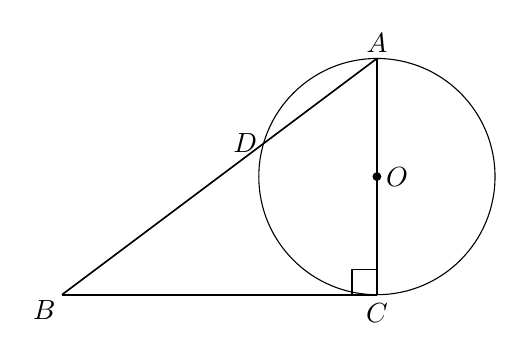
\begin{tikzpicture}[semithick, line join=round]
  \coordinate (C) at (0,0);
  \coordinate (A) at (0,3);
  \coordinate (B) at (-4,0);
  \coordinate (O) at (0,1.5);
  \coordinate (D) at (-1.44,1.92);

  % 以 AC 为直径的圆
  \draw[thin] (O) circle (1.5);

  % 三角形三边
  \draw (A) -- (B);
  \draw (B) -- (C);
  \draw (C) -- (A);

  % C 处直角符号
  \draw (0,0.32) -- (-0.32,0.32) -- (-0.32,0);

  % 圆心
  \fill (O) circle (1.6pt);

  % 顶点与交点标注
  \node[above, inner sep=2pt] at (A) {$A$};
  \node[below left, inner sep=2pt] at (B) {$B$};
  \node[below, inner sep=3pt] at (C) {$C$};
  \node[right, inner sep=3pt] at (O) {$O$};
  \node[left, inner sep=2pt] at (D) {$D$};
\end{tikzpicture}
\end{center}
\nopagebreak[4]
【C】参数方程 $\begin{cases}x=\cos\alpha,\\[2pt]y=1+\sin\alpha,\end{cases}$（$\alpha$ 为参数）化成普通方程为 $\underline{\qquad}$．

\Needspace{4\baselineskip}
\textbf{解析}

\Needspace{5\baselineskip}
\textbf{【A】} 由 $|2x-1|<3$ 得
\nopagebreak[4]
\[-3<2x-1<3.\]
各边加 $1$：$-2<2x<4$；再除以 $2$：$-1<x<2$。故解集为 $(-1,2)$。
代回检验：$x=0$ 时 $|{-1}|=1<3$，成立；端点 $x=-1$ 时 $|{-3}|=3$，不满足严格小于；$x=2$ 时 $|3|=3$，同样不满足。

\textbf{【B】} 【图注】原页图中 $A$ 在最高处，$C$ 在其正下方（直角顶点，直角符号画在 $C$ 的内侧），$B$ 在左下方，圆以 $AC$ 为直径且向右鼓出 $AC$ 之外，$D$ 在 $A$ 与 $B$ 之间。

\Needspace{5\baselineskip}
$\angle ACB=90^\circ$，$AC=3$，$BC=4$，故
\nopagebreak[4]
\[AB=\sqrt{3^2+4^2}=5.\]
\Needspace{5\baselineskip}
因 $AC$ 为直径、$D$ 在圆周上，由直径所对的圆周角为直角得 $\angle ADC=90^\circ$，即 $CD\perp AB$。于是直角边 $BC$ 在斜边 $AB$ 上的射影为 $BD$，由射影定理
\nopagebreak[4]
\[BC^2=BD\cdot AB\ \Longrightarrow\ BD=\frac{BC^2}{AB}=\frac{16}{5}.\]
核对：另一条直角边 $AC$ 的射影 $AD=\dfrac{AC^2}{AB}=\dfrac95$，而 $AD+BD=\dfrac95+\dfrac{16}{5}=5=AB$，相符；且 $CD^2=AD\cdot BD=\dfrac95\cdot\dfrac{16}{5}=\dfrac{144}{25}$，$CD=\dfrac{12}{5}$，与 $CD=\dfrac{AC\cdot BC}{AB}=\dfrac{12}{5}$ 一致。

\Needspace{5\baselineskip}
\textbf{【C】} 由参数方程
\nopagebreak[4]
\[\begin{cases}x=\cos\alpha,\\ y=1+\sin\alpha,\end{cases}\]
\Needspace{5\baselineskip}
得 $\cos\alpha=x$，$\sin\alpha=y-1$。两式平方相加，利用 $\cos^2\alpha+\sin^2\alpha=1$：
\nopagebreak[4]
\[x^2+(y-1)^2=1.\]
这就是所求的普通方程（表示圆心 $(0,1)$、半径 $1$ 的圆）。
代回检验：$\alpha=0$ 时 $(x,y)=(1,1)$，满足 $1+0=1$；$\alpha=\dfrac\pi2$ 时 $(0,2)$，满足 $0+1=1$；$\alpha=\pi$ 时 $(-1,1)$，满足 $1+0=1$。

\gkanswer{答案：【A】$(-1,2)$；【B】$\dfrac{16}{5}$；【C】$x^2+(y-1)^2=1$。}

\end{answer}
\begin{answer}
\gksolhead{16}{}

\textbf{题目}：

已知 $\{a_n\}$ 是公差不为零的等差数列，$a_1=1$ 且 $a_1$，$a_3$，$a_9$ 成等比数列．

（1）求数列 $\{a_n\}$ 的通项；

（2）求数列 $\{2^{a_n}\}$ 的前 $n$ 项和 $S_n$．

\Needspace{4\baselineskip}
\textbf{解析}

\Needspace{5\baselineskip}
（1）设公差为 $d$，由 $a_1=1$ 得
\nopagebreak[4]
\[a_3=1+2d,\qquad a_9=1+8d.\]
\Needspace{5\baselineskip}
$a_1$，$a_3$，$a_9$ 成等比数列，故 $a_3^2=a_1a_9$：
\nopagebreak[4]
\[(1+2d)^2=1\cdot(1+8d)\ \Longrightarrow\ 1+4d+4d^2=1+8d\ \Longrightarrow\ 4d^2-4d=0,\]
\Needspace{5\baselineskip}
即 $4d(d-1)=0$。由「公差不为零」得 $d\ne 0$，故 $d=1$。于是
\nopagebreak[4]
\[a_n=1+(n-1)\cdot 1=n.\]

\Needspace{5\baselineskip}
（2）由（1）$2^{a_n}=2^n$，这是首项 $2$、公比 $2$ 的等比数列，前 $n$ 项和
\nopagebreak[4]
\[S_n=\frac{2(2^n-1)}{2-1}=2^{n+1}-2.\]
验算：$n=1$ 时 $S_1=2$，公式给 $2^2-2=2$；$n=2$ 时 $S_2=2+4=6$，公式给 $2^3-2=6$，相符。

\gkanswer{答案：（1）$a_n=n$；（2）$S_n=2^{n+1}-2$。}

\end{answer}
\begin{answer}
\gksolhead{17}{}

\textbf{题目}：

如图，在 $\triangle ABC$ 中，已知 $\angle B=45^\circ$，$D$ 是 $BC$ 边上的一点，$AD=10$，$AC=14$，$DC=6$，求 $AB$ 的长．
\nopagebreak[4]
\begin{center}% 2010 年陕西卷文科第 17 题：△ABC 中 D 在 BC 上，已知 ∠B=45°、AD=10、AC=14、DC=6。
% 来源 PDF：普通高考/2010/2010陕西文.pdf，SHA-256 428bcb4aee4c6a7a6a9c9d0dca1377b14112594015d1d50a931e725ae0c5c130。
% 原页：第 1 页（A3 三栏）第 3 栏下部，书页码 625。
% 重绘依据：照原页——B 在左下、C 在右下，BC 水平；A 在 BC 上方、位于 B 与 D 之间偏 D 一侧；
%   D 在 BC 上（介于 B、C 之间），连 AD、AC，只有 AB、AD、AC、BC 四条实线，无其他辅助线。
%   按题设取坐标（整体缩小 1/2.5）：B=(0,0)，A=(3.464,3.464)（∠B=45°），
%   D=(5.464,0)，C=(7.864,0)，此时 AD=4、DC=2.4、AC=5.6，与原图比例一致。
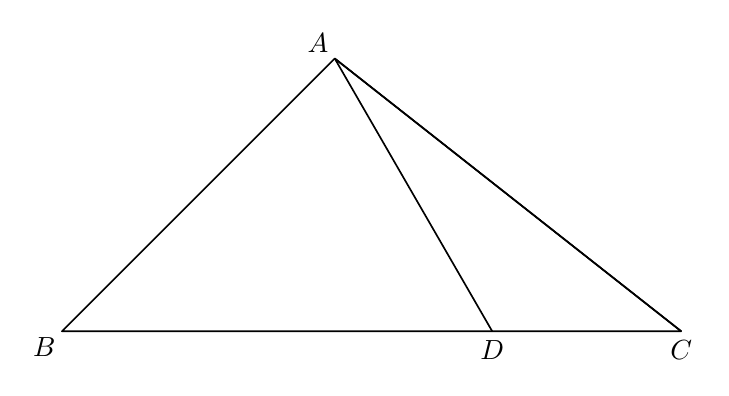
\begin{tikzpicture}[semithick, line join=round]
  \coordinate (B) at (0,0);
  \coordinate (C) at (7.864,0);
  \coordinate (D) at (5.464,0);
  \coordinate (A) at (3.464,3.464);

  \draw (A) -- (B) -- (C) -- cycle;
  \draw (A) -- (D);
  \draw (A) -- (C);

  \node[above left, inner sep=2pt] at (A) {$A$};
  \node[below left, inner sep=2pt] at (B) {$B$};
  \node[below, inner sep=3pt] at (C) {$C$};
  \node[below, inner sep=3pt] at (D) {$D$};
\end{tikzpicture}
\end{center}
\nopagebreak[4]
\Needspace{4\baselineskip}
\textbf{解析}

【图注】原页图中 $B$ 在左下、$C$ 在右下，$BC$ 水平；$A$ 在 $BC$ 上方偏右，$D$ 在 $BC$ 上且介于 $B$、$C$ 之间；连 $AB$、$AD$、$AC$，无其他辅助线。

\Needspace{5\baselineskip}
先在 $\triangle ADC$ 中用余弦定理求 $\angle ADC$。三边 $AD=10$，$DC=6$，$AC=14$：
\nopagebreak[4]
\[\cos\angle ADC=\frac{AD^2+DC^2-AC^2}{2\cdot AD\cdot DC}=\frac{100+36-196}{2\times 10\times 6}=\frac{-60}{120}=-\frac12,\]
\Needspace{5\baselineskip}
故 $\angle ADC=120^\circ$。因 $B$，$D$，$C$ 共线且 $D$ 在 $B$、$C$ 之间，$\angle ADB$ 与 $\angle ADC$ 互为邻补角：
\nopagebreak[4]
\[\angle ADB=180^\circ-120^\circ=60^\circ.\]
\Needspace{5\baselineskip}
在 $\triangle ABD$ 中，已知 $\angle B=45^\circ$，$\angle ADB=60^\circ$，$AD=10$。由正弦定理
\nopagebreak[4]
\[\frac{AB}{\sin\angle ADB}=\frac{AD}{\sin B}\ \Longrightarrow\ AB=\frac{AD\sin\angle ADB}{\sin B}=\frac{10\sin 60^\circ}{\sin 45^\circ}=\frac{10\cdot\frac{\sqrt3}{2}}{\frac{\sqrt2}{2}}=5\sqrt6.\]
\Needspace{5\baselineskip}
另路核对：在 $\triangle ADC$ 中由正弦定理 $\dfrac{AC}{\sin\angle ADC}=\dfrac{AD}{\sin C}$，得
\nopagebreak[4]
\[\sin C=\frac{10\cdot\frac{\sqrt3}{2}}{14}=\frac{5\sqrt3}{14},\qquad \cos C=\sqrt{1-\frac{75}{196}}=\frac{11}{14}.\]
\Needspace{5\baselineskip}
再用 $\triangle ABC$ 的正弦定理 $\dfrac{AB}{\sin C}=\dfrac{AC}{\sin 45^\circ}$：
\nopagebreak[4]
\[AB=14\cdot\frac{5\sqrt3}{14}\cdot\sqrt2=5\sqrt6,\]
与上面一致。

\gkanswer{答案：$5\sqrt6$。}

\end{answer}
\begin{answer}
\gksolhead{18}{}

\textbf{题目}：

如图，在四棱锥 $P-ABCD$ 中，底面 $ABCD$ 是矩形，$PA\perp$ 平面 $ABCD$，$AP=AB=2$，$BC=2\sqrt2$，$E$，$F$ 分别是 $AD$，$PC$ 的中点．

（1）证明：$PC\perp$ 平面 $BEF$；

（2）求平面 $BEF$ 与平面 $BAP$ 夹角的大小．
\nopagebreak[4]
\begin{center}% 2010 年陕西卷文科第 18 题：四棱锥 P-ABCD 与平面 BEF。
% 来源 PDF：普通高考/2010/2010陕西文.pdf，SHA-256 428bcb4aee4c6a7a6a9c9d0dca1377b14112594015d1d50a931e725ae0c5c130。
% 原页：第 2 页（A3 三栏）第 1 栏上部，书页码 626。
% 重绘依据：照原页——P 在最高处、A 在其正下方（A 为被遮挡的后角，故 PA 画虚线），
%   B 在左下、C 在右下、D 在右侧与 A 同一水平高度；矩形 ABCD 中 AB、AD 为被遮挡的边（虚线），
%   BC、CD 为可见边（实线）；PB、PC、PD 为可见棱（实线）。
%   E 为 AD 中点、F 为 PC 中点：BF 落在可见侧面 PBC 内（实线），BE、EF 为体内辅助线（虚线）。
%   坐标（cm）：B=(0,0)，C=(6.4,0)，A=(1.9,2.3)，D=(8.3,2.3)，P=(2.0,7.6)，
%   则 E=(5.1,2.3)，F=(4.2,3.8)。
\begin{tikzpicture}[semithick, line join=round]
  \coordinate (B) at (0,0);
  \coordinate (C) at (6.4,0);
  \coordinate (A) at (1.9,2.3);
  \coordinate (D) at (8.3,2.3);
  \coordinate (P) at (2.0,7.6);
  \coordinate (E) at (5.1,2.3);
  \coordinate (F) at (4.2,3.8);

  % 可见棱与可见底边（实线）
  \draw (P) -- (B);
  \draw (P) -- (C);
  \draw (P) -- (D);
  \draw (B) -- (C);
  \draw (C) -- (D);
  \draw (B) -- (F);

  % 被遮挡的棱与体内辅助线（虚线）
  \draw[dashed] (P) -- (A);
  \draw[dashed] (A) -- (B);
  \draw[dashed] (A) -- (D);
  \draw[dashed] (B) -- (E);
  \draw[dashed] (E) -- (F);

  % 中点记号
  \draw ($(E)!0.055cm!90:(A)$) -- ($(E)!-0.055cm!90:(A)$);
  \draw ($(F)!0.055cm!90:(P)$) -- ($(F)!-0.055cm!90:(P)$);

  % 顶点标注
  \node[above, inner sep=2pt] at (P) {$P$};
  \node[above left, inner sep=1pt] at (A) {$A$};
  \node[below left, inner sep=2pt] at (B) {$B$};
  \node[below right, inner sep=2pt] at (C) {$C$};
  \node[right, inner sep=3pt] at (D) {$D$};
  \node[below, inner sep=3pt] at (E) {$E$};
  \node[right, inner sep=3pt] at (F) {$F$};
\end{tikzpicture}
\end{center}
\nopagebreak[4]
\Needspace{4\baselineskip}
\textbf{解析}

【图注】原页图中 $P$ 在最高处，$A$ 在 $P$ 正下方（后侧被遮挡的角，故 $PA$ 画虚线），$B$ 在左下、$C$ 在右下，$D$ 在右侧与 $A$ 同高；矩形 $ABCD$ 中 $AB$、$AD$ 为被遮挡的边（虚线），$BC$、$CD$ 为可见边（实线）；$E$ 为 $AD$ 中点、$F$ 为 $PC$ 中点，$BF$ 在可见侧面内画实线，$BE$、$EF$ 为体内辅助线（虚线）。

\Needspace{5\baselineskip}
（1）以 $A$ 为原点，$\overrightarrow{AB}$、$\overrightarrow{AD}$、$\overrightarrow{AP}$ 的方向分别为 $x$、$y$、$z$ 轴建立空间直角坐标系。由 $AP=AB=2$，$BC=AD=2\sqrt2$ 得
\nopagebreak[4]
\[A(0,0,0),\ B(2,0,0),\ C(2,2\sqrt2,0),\ D(0,2\sqrt2,0),\ P(0,0,2).\]
\Needspace{5\baselineskip}
$E$ 是 $AD$ 中点，$F$ 是 $PC$ 中点，故
\nopagebreak[4]
\[E(0,\sqrt2,0),\qquad F\left(\frac{2+0}{2},\frac{2\sqrt2+0}{2},\frac{0+2}{2}\right)=(1,\sqrt2,1).\]
\Needspace{5\baselineskip}
于是
\nopagebreak[4]
\[\overrightarrow{PC}=(2,2\sqrt2,-2),\quad \overrightarrow{BE}=(-2,\sqrt2,0),\quad \overrightarrow{BF}=(-1,\sqrt2,1).\]
\Needspace{5\baselineskip}
计算内积：
\nopagebreak[4]
\[\overrightarrow{PC}\cdot\overrightarrow{BE}=2\times(-2)+2\sqrt2\times\sqrt2+(-2)\times 0=-4+4+0=0,\]
\nopagebreak[4]
\[\overrightarrow{PC}\cdot\overrightarrow{BF}=2\times(-1)+2\sqrt2\times\sqrt2+(-2)\times 1=-2+4-2=0.\]
\Needspace{5\baselineskip}
故 $PC\perp BE$，$PC\perp BF$。又 $BE$ 与 $BF$ 是平面 $BEF$ 内两条相交直线（交于 $B$），所以
\nopagebreak[4]
\[PC\perp\text{\text{平面} }BEF.\]

\Needspace{5\baselineskip}
（2）平面 $BAP$ 由 $A(0,0,0)$、$B(2,0,0)$、$P(0,0,2)$ 确定，即 $y=0$ 平面，法向量
\nopagebreak[4]
\[\boldsymbol n_1=(0,1,0).\]
\Needspace{5\baselineskip}
平面 $BEF$ 的法向量可取
\nopagebreak[4]
\[\boldsymbol n_2=\overrightarrow{BE}\times\overrightarrow{BF}=\begin{vmatrix}\boldsymbol i&\boldsymbol j&\boldsymbol k\\ -2&\sqrt2&0\\ -1&\sqrt2&1\end{vmatrix}=(\sqrt2-0,\ 0-(-2),\ -2\sqrt2+\sqrt2)=(\sqrt2,\,2,\,-\sqrt2).\]
\Needspace{5\baselineskip}
设两平面夹角为 $\theta$，则
\nopagebreak[4]
\[\cos\theta=\frac{|\boldsymbol n_1\cdot\boldsymbol n_2|}{|\boldsymbol n_1||\boldsymbol n_2|}=\frac{2}{1\times\sqrt{2+4+2}}=\frac{2}{2\sqrt2}=\frac{\sqrt2}{2},\]
故 $\theta=45^\circ$，即平面 $BEF$ 与平面 $BAP$ 的夹角为 $45^\circ$。

\gkanswer{答案：（1）证明见解析；（2）$45^\circ$。}

\end{answer}
\begin{answer}
\gksolhead{19}{}

\textbf{题目}：

为了解学生身高情况，某校以 $10\%$ 的比例对全校 $700$ 名学生按性别进行分层抽样调查，测得身高情况的统计图如下：

（1）估计该校男生的人数；

（2）估计该校学生身高在 $170\sim 185\ \mathrm{cm}$ 之间的概率；

（3）从样本中身高在 $165\sim 180\ \mathrm{cm}$ 之间的女生中任选 $2$ 人，求至少有 $1$ 人身高在 $170\sim 180\ \mathrm{cm}$ 之间的概率．
\nopagebreak[4]
\begin{center}% 2010 年陕西卷文科第 19 题：男、女生身高频数分布直方图（样本各 40 人、30 人）。
% 来源 PDF：普通高考/2010/2010陕西文.pdf，SHA-256 428bcb4aee4c6a7a6a9c9d0dca1377b14112594015d1d50a931e725ae0c5c130。
% 原页：第 2 页（A3 三栏）第 1 栏下部，书页码 626。
% 重绘依据：照原页——左「男生」、右「女生」两幅频数直方图，横轴 身高/cm 自 160 起每 5 cm 一组
%   至 190，纵轴为频数（原点处画有断裂符号）。
%   男生各组频数依次为 2, 5, 14, 13, 4, 2（合计 40）；女生依次为 1, 7, 12, 6, 3, 1（合计 30）。
%   原页在各组上沿引出水平虚线并标注频数：男生 14、13、5、4、2；女生 12、7、6、3、1。
\begin{tikzpicture}[x=0.62cm, y=0.30cm, semithick, line join=round,
  lbl/.style={font=\scriptsize, inner sep=1pt}]

  % ================= 男生 =================
  \begin{scope}
    % 坐标轴
    \draw[->, >=stealth] (-0.55,-1.20) -- (-0.55,16.00);
    \draw[->, >=stealth] (-1.20,0) -- (7.05,0);
    \node[lbl, right] at (-0.60,14.75) {频数};
    \node[lbl, above] at (6.40,1.00) {身高/cm};

    % 原点断裂符号
    \draw[thin] (-0.98,0) -- (-0.90,1.10) -- (-0.82,-1.10) -- (-0.74,1.10) -- (-0.66,0);
    \node[lbl, below] at (-1.02,-0.20) {$0$};

    % 各组矩形
    \foreach \i/\h in {0/2, 1/5, 2/14, 3/13, 4/4, 5/2} {
      \draw (\i,0) rectangle (\i+1,\h);
    }

    % 频数虚线（自纵轴引到该频数组的左沿）
    \foreach \i/\h in {0/2, 1/5, 2/14, 3/13, 4/4} {
      \draw[thin, dashed] (-0.55,\h) -- (\i,\h);
    }
    \node[lbl, left] at (-0.62,2) {$2$};
    \node[lbl, left] at (-0.62,5) {$5$};
    \node[lbl, left] at (-0.62,4) {$4$};
    \node[lbl, left] at (-0.62,14) {$14$};
    \node[lbl, left] at (-0.62,13) {$13$};

    % 横轴刻度
    \foreach \i/\v in {0/160, 1/165, 2/170, 3/175, 4/180, 5/185, 6/190} {
      \draw[thin] (\i,0) -- (\i,-0.90);
      \node[lbl, below] at (\i,-1.05) {\v};
    }

    % 标题
    \node at (3.0,17.30) {男生};
  \end{scope}

  % ================= 女生 =================
  \begin{scope}[xshift=5.35cm]
    \draw[->, >=stealth] (-0.55,-1.20) -- (-0.55,16.00);
    \draw[->, >=stealth] (-1.20,0) -- (7.05,0);
    \node[lbl, right] at (-0.60,14.75) {频数};
    \node[lbl, above] at (6.40,1.00) {身高/cm};

    \draw[thin] (-0.98,0) -- (-0.90,1.10) -- (-0.82,-1.10) -- (-0.74,1.10) -- (-0.66,0);
    \node[lbl, below] at (-1.02,-0.20) {$0$};

    \foreach \i/\h in {0/1, 1/7, 2/12, 3/6, 4/3, 5/1} {
      \draw (\i,0) rectangle (\i+1,\h);
    }

    \foreach \i/\h in {0/1, 1/7, 2/12, 3/6, 4/3} {
      \draw[thin, dashed] (-0.55,\h) -- (\i,\h);
    }
    \node[lbl, left] at (-0.62,1) {$1$};
    \node[lbl, left] at (-0.62,7) {$7$};
    \node[lbl, left] at (-0.62,6) {$6$};
    \node[lbl, left] at (-0.62,12) {$12$};
    \node[lbl, left] at (-0.62,3) {$3$};

    \foreach \i/\v in {0/160, 1/165, 2/170, 3/175, 4/180, 5/185, 6/190} {
      \draw[thin] (\i,0) -- (\i,-0.90);
      \node[lbl, below] at (\i,-1.05) {\v};
    }

    \node at (3.0,17.30) {女生};
  \end{scope}
\end{tikzpicture}
\end{center}
\nopagebreak[4]
\Needspace{4\baselineskip}
\textbf{解析}

【图注】原页并排两幅频数直方图，左标「男生」、右标「女生」，横轴为身高/cm，自 $160$ 起每 $5\ \mathrm{cm}$ 一组至 $190$，纵轴为频数，原点处画有断裂符号，各组上沿引出水平虚线并标注频数。

\Needspace{5\baselineskip}
读图得各组频数：
\nopagebreak[4]
\[\text{\text{男生}}:\ 2,\ 5,\ 14,\ 13,\ 4,\ 2\quad(\text{\text{合计} }40);\qquad \text{\text{女生}}:\ 1,\ 7,\ 12,\ 6,\ 3,\ 1\quad(\text{\text{合计} }30).\]
样本容量 $700\times 10\%=70$，恰为 $40+30$，说明读图无误。

\Needspace{5\baselineskip}
（1）男生在样本中占 $\dfrac{40}{70}$，按分层抽样，全校男生约占
\nopagebreak[4]
\[700\times\frac{40}{70}=400\ (\text{\text{人}}).\]

\Needspace{5\baselineskip}
（2）身高在 $170\sim 185\ \mathrm{cm}$ 的样本人数为
\nopagebreak[4]
\[\text{\text{男生}}\ 14+13+4=31,\qquad \text{\text{女生}}\ 12+6+3=21,\]
\Needspace{5\baselineskip}
共 $52$ 人。用样本频率估计概率：
\nopagebreak[4]
\[P\approx\frac{52}{70}=\frac{26}{35}.\]

\Needspace{5\baselineskip}
（3）身高在 $165\sim 180\ \mathrm{cm}$ 的女生即 $[165,170)$、$[170,175)$、$[175,180)$ 三组，共
\nopagebreak[4]
\[7+12+6=25\ (\text{\text{人}}),\]
其中身高在 $170\sim 180\ \mathrm{cm}$ 的（即后两组）有 $12+6=18$ 人，在 $[165,170)$ 的有 $7$ 人。

\Needspace{5\baselineskip}
从这 $25$ 人中任选 $2$ 人，每种选法等可能，共
\nopagebreak[4]
\[\mathrm C_{25}^2=\frac{25\times 24}{2}=300\ (\text{\text{种}}).\]
\Needspace{5\baselineskip}
「至少有 $1$ 人身高在 $170\sim 180\ \mathrm{cm}$」的对立事件是「两人身高都在 $[165,170)$」，后者有
\nopagebreak[4]
\[\mathrm C_7^2=\frac{7\times 6}{2}=21\ (\text{\text{种}}).\]
\Needspace{5\baselineskip}
故所求概率
\nopagebreak[4]
\[P=1-\frac{21}{300}=\frac{279}{300}=\frac{93}{100}.\]
核对：也可正面算——恰有 $1$ 人在 $170\sim 180$ 的情形有 $\mathrm C_{18}^1\mathrm C_7^1=126$ 种，两人都在 $170\sim 180$ 的有 $\mathrm C_{18}^2=153$ 种，合计 $126+153=279$，与 $300-21=279$ 一致。
\Needspace{5\baselineskip}
按基本事件逐个计概率再求和：任取 $2$ 人的每一种选法（基本事件）等可能，概率都是 $\dfrac{1}{300}$，其中使「至少有 $1$ 人在 $170\sim 180$」的选法有 $279$ 种且互不相容，故
\nopagebreak[4]
\[P=\sum_{\text{279 \text{个互不相容的有利基本事件}}}\frac{1}{300}=279\times\frac{1}{300}=\frac{93}{100}.\]

\gkanswer{答案：（1）$400$；（2）$\dfrac{26}{35}$；（3）$\dfrac{93}{100}$。}

\end{answer}
\begin{answer}
\gksolhead{20}{}

\textbf{题目}：

如图，椭圆 $C:\dfrac{x^2}{a^2}+\dfrac{y^2}{b^2}=1$ 的顶点为 $A_1$，$A_2$，$B_1$，$B_2$，焦点为 $F_1$，$F_2$，$|A_1B_1|=\sqrt7$，$S_{\square A_1B_1A_2B_2}=2S_{\square B_1F_1B_2F_2}$．

（1）求椭圆 $C$ 的方程；

（2）设 $n$ 是过原点的直线，$l$ 是与 $n$ 垂直相交于 $P$ 点、与椭圆相交于 $A$，$B$ 两点的直线，$|\overrightarrow{OP}|=1$．是否存在上述直线 $l$ 使 $\overrightarrow{AP}\cdot\overrightarrow{PB}=1$ 成立？若存在，求出直线 $l$ 的方程；若不存在，请说明理由．
\nopagebreak[4]
\begin{center}% 2010 年陕西卷文科第 20 题：椭圆 C 与过原点直线 n、与之垂直的直线 l。
% 来源 PDF：普通高考/2010/2010陕西文.pdf，SHA-256 428bcb4aee4c6a7a6a9c9d0dca1377b14112594015d1d50a931e725ae0c5c130。
% 原页：第 2 页（A3 三栏）第 2 栏中部，书页码 626。
% 重绘依据：照原页——椭圆中心为 O，长短轴端点为 A1（左）、A2（右）、B1（上）、B2（下），
%   两焦点 F1（左）、F2（右）用圆点标出；直线 n 过 O 斜向右上到 P，直线 l 过 P 且与 n 垂直，
%   在 P 处画直角符号；l 与椭圆交于右上的 A、右下的 B，并在 A、B 之外略作延长。
%   按 (1) 的结论 a=2、b=√3 取图（整体乘 1.5）：A1=(-3,0)，A2=(3,0)，B1=(0,2.598)，B2=(0,-2.598)，
%   F1=(-1.5,0)，F2=(1.5,0)；再取 |OP|=1.5、n 的倾角约 18.4°，得 P=(1.423,0.474)，
%   l: y=-3x+4.743，与椭圆交于 A=(0.742,2.517)、B=(2.177,-1.788)。
\begin{tikzpicture}[semithick, line join=round]
  \coordinate (O)  at (0,0);
  \coordinate (A1) at (-3,0);
  \coordinate (A2) at (3,0);
  \coordinate (B1) at (0,{1.5*sqrt(3)});
  \coordinate (B2) at (0,{-1.5*sqrt(3)});
  \coordinate (F1) at (-1.5,0);
  \coordinate (F2) at (1.5,0);
  \coordinate (P)  at (1.423,0.474);
  \coordinate (A)  at (0.742,2.517);
  \coordinate (B)  at (2.177,-1.788);

  % 坐标轴
  \draw[->, >=stealth] (-4.10,0) -- (4.30,0) node[below, inner sep=3pt] {$x$};
  \draw[->, >=stealth] (0,-3.70) -- (0,3.60) node[left, inner sep=3pt] {$y$};

  % 椭圆
  \draw plot[domain=0:360, samples=160] ({3*cos(\x)}, {1.5*sqrt(3)*sin(\x)});

  % 直线 l（在 A、B 之外略作延长）
  \draw (0.62,2.88) -- (2.35,-2.31);

  % 直线 n：O 到 P
  \draw (O) -- (P);

  % P 处直角符号（n ⊥ l）
  \coordinate (Pu) at ($(P)!0.32cm!(A)$);
  \coordinate (Pv) at ($(P)!0.32cm!(O)$);
  \draw ($(Pu)+(Pv)-(P)$) -- (Pu);
  \draw ($(Pu)+(Pv)-(P)$) -- (Pv);

  % 焦点圆点
  \fill (F1) circle (1.7pt);
  \fill (F2) circle (1.7pt);

  % 标注
  \node[below left, inner sep=2pt] at (A1) {$A_1$};
  \node[below right, inner sep=2pt] at (A2) {$A_2$};
  \node[above left, inner sep=2pt] at (B1) {$B_1$};
  \node[below left, inner sep=2pt] at (B2) {$B_2$};
  \node[below, inner sep=3pt] at (F1) {$F_1$};
  \node[below, inner sep=3pt] at (F2) {$F_2$};
  \node[left, inner sep=3pt] at (O) {$O$};
  \node[right, inner sep=3pt] at (P) {$P$};
  \node[right, inner sep=2pt] at (A) {$A$};
  \node[left, inner sep=3pt] at (B) {$B$};
  \node[above left, inner sep=3pt] at (1.05,0.55) {$n$};
  \node[above left, inner sep=2pt] at (0.60,2.92) {$l$};
\end{tikzpicture}
\end{center}
\nopagebreak[4]
\Needspace{4\baselineskip}
\textbf{解析}

【图注】原页图中椭圆中心为 $O$，长短轴端点为 $A_1$（左）、$A_2$（右）、$B_1$（上）、$B_2$（下），焦点 $F_1$（左）、$F_2$（右）用圆点标出；直线 $n$ 过 $O$ 斜向右上至 $P$，直线 $l$ 过 $P$ 且与 $n$ 垂直（$P$ 处画直角符号），$l$ 与椭圆交于右上的 $A$ 与右下的 $B$。

\Needspace{5\baselineskip}
（1）记 $c=\sqrt{a^2-b^2}$。$A_1(-a,0)$、$B_1(0,b)$，故
\nopagebreak[4]
\[|A_1B_1|=\sqrt{a^2+b^2}=\sqrt7.\]
\Needspace{5\baselineskip}
菱形 $A_1B_1A_2B_2$ 的对角线为 $A_1A_2=2a$、$B_1B_2=2b$，面积
\nopagebreak[4]
\[S_{\square A_1B_1A_2B_2}=\frac12\cdot 2a\cdot 2b=2ab.\]
\Needspace{5\baselineskip}
菱形 $B_1F_1B_2F_2$ 的对角线为 $B_1B_2=2b$、$F_1F_2=2c$，面积
\nopagebreak[4]
\[S_{\square B_1F_1B_2F_2}=\frac12\cdot 2b\cdot 2c=2bc.\]
\Needspace{5\baselineskip}
由题设 $2ab=2\cdot 2bc$，即 $a=2c$。于是
\nopagebreak[4]
\[b^2=a^2-c^2=4c^2-c^2=3c^2,\qquad a^2+b^2=4c^2+3c^2=7c^2=7,\]
\Needspace{5\baselineskip}
得 $c=1$，$a=2$，$b=\sqrt3$，椭圆方程为
\nopagebreak[4]
\[\frac{x^2}{4}+\frac{y^2}{3}=1.\]

（2）$l\perp n$ 于 $P$，而 $n$ 过原点，所以 $P$ 是原点 $O$ 到直线 $l$ 的垂足，$|\overrightarrow{OP}|=1$ 即 $O$ 到 $l$ 的距离为 $1$。又 $1<\sqrt3=b$，故 $P$ 在椭圆内部，$l$ 与椭圆必有两个交点。

\Needspace{5\baselineskip}
设 $P=(x_0,y_0)$，则 $x_0^2+y_0^2=1$。因 $l\perp OP$，$l$ 的一个单位方向向量为 $\boldsymbol u=(-y_0,x_0)$，$l$ 上的点可写成 $P+s\boldsymbol u$，即
\nopagebreak[4]
\[(x,y)=(x_0-sy_0,\ y_0+sx_0).\]
\Needspace{5\baselineskip}
代入椭圆方程 $\dfrac{x^2}{4}+\dfrac{y^2}{3}=1$：
\nopagebreak[4]
\[\frac{(x_0-sy_0)^2}{4}+\frac{(y_0+sx_0)^2}{3}=1.\]
\Needspace{5\baselineskip}
展开整理，关于 $s$ 的二次项系数与常数项分别为
\nopagebreak[4]
\[A=\frac{y_0^2}{4}+\frac{x_0^2}{3},\qquad C=\frac{x_0^2}{4}+\frac{y_0^2}{3}.\]
\Needspace{5\baselineskip}
设 $A$、$B$ 两点对应的参数为 $s_1$、$s_2$，则 $s_1s_2=\dfrac{C-1}{A}$。$P$ 在椭圆内部，故 $A$、$B$ 分居 $P$ 两侧，$s_1$、$s_2$ 异号，于是
\nopagebreak[4]
\[\overrightarrow{AP}\cdot\overrightarrow{PB}=|\overrightarrow{AP}|\cdot|\overrightarrow{PB}|=|s_1|\cdot|s_2|=-s_1s_2=\frac{1-C}{A}.\]
\Needspace{5\baselineskip}
用 $x_0^2=1-y_0^2$ 化简：
\nopagebreak[4]
\[C=\frac{1-y_0^2}{4}+\frac{y_0^2}{3}=\frac14+\frac{y_0^2}{12},\qquad A=\frac{y_0^2}{4}+\frac{1-y_0^2}{3}=\frac13-\frac{y_0^2}{12},\]
\Needspace{5\baselineskip}
故
\nopagebreak[4]
\[\overrightarrow{AP}\cdot\overrightarrow{PB}=\frac{\frac34-\frac{y_0^2}{12}}{\frac13-\frac{y_0^2}{12}}=\frac{9-y_0^2}{4-y_0^2}=1+\frac{5}{4-y_0^2}.\]
\Needspace{5\baselineskip}
其中 $0\leqslant y_0^2\leqslant 1$，故 $\dfrac{5}{4-y_0^2}$ 随 $y_0^2$ 增大而增大，取值范围是 $\left[\dfrac54,\dfrac53\right]$，从而
\nopagebreak[4]
\[\frac94\leqslant\overrightarrow{AP}\cdot\overrightarrow{PB}\leqslant\frac83.\]
恒不等于 $1$。

\Needspace{5\baselineskip}
用斜截式另核一遍（斜率存在时）：设 $l:y=kx+t$，由 $\dfrac{|t|}{\sqrt{1+k^2}}=1$ 得 $t^2=1+k^2$。代入椭圆得 $(3+4k^2)x^2+8ktx+4t^2-12=0$，设 $A(x_1,y_1)$、$B(x_2,y_2)$，则 $x_1+x_2=-\dfrac{8kt}{3+4k^2}$，$x_1x_2=\dfrac{4t^2-12}{3+4k^2}$，而 $P$ 的横坐标 $x_0=-\dfrac{kt}{1+k^2}$。同法算得
\nopagebreak[4]
\[\overrightarrow{AP}\cdot\overrightarrow{PB}=(1+k^2)\left|x_1x_2-x_0(x_1+x_2)+x_0^2\right|=\frac{8+9k^2}{3+4k^2},\]
与上式的对应关系由 $y_0^2=\dfrac{1}{1+k^2}$（$P$ 为原点到 $y=kx+t$ 的垂足，且 $t^2=1+k^2$）给出：$\dfrac{9-y_0^2}{4-y_0^2}=\dfrac{9(1+k^2)-1}{4(1+k^2)-1}=\dfrac{8+9k^2}{3+4k^2}$，两路一致。$k=0$（$l$ 为 $y=\pm1$）时 $y_0^2=1$，得 $\dfrac83$；$k\to\infty$（$l$ 为 $x=\pm1$）时 $y_0^2\to0$，得 $\dfrac94$，即上面的上下界。
故不存在满足 $\overrightarrow{AP}\cdot\overrightarrow{PB}=1$ 的直线 $l$。

\gkanswer{答案：（1）$\dfrac{x^2}{4}+\dfrac{y^2}{3}=1$；（2）不存在。}

\end{answer}
\begin{answer}
\gksolhead{21}{}

\textbf{题目}：

已知函数 $f(x)=\sqrt x$，$g(x)=a\ln x$，$a\in\mathbf R$．

（1）若曲线 $y=f(x)$ 与曲线 $y=g(x)$ 相交，且在交点处有共同的切线，求 $a$ 的值和该切线方程；

（2）设函数 $h(x)=f(x)-g(x)$，当 $h(x)$ 存在最小值时，求其最小值 $\varphi(a)$ 的解析式；

（3）对（2）中的 $\varphi(a)$ 和任意的 $a>0$，$b>0$，证明：$\varphi'\left(\dfrac{a+b}{2}\right)\leqslant\dfrac{\varphi'(a)+\varphi'(b)}{2}\leqslant\varphi'\left(\dfrac{2ab}{a+b}\right)$．

\Needspace{4\baselineskip}
\textbf{解析}

\Needspace{5\baselineskip}
（1）设两曲线交点横坐标为 $x_0>0$。交点处函数值相等、切线斜率相等：
\nopagebreak[4]
\[\sqrt{x_0}=a\ln x_0,\qquad \frac{1}{2\sqrt{x_0}}=\frac{a}{x_0}.\]
\Needspace{5\baselineskip}
由第二式得 $a=\dfrac{x_0}{2\sqrt{x_0}}=\dfrac{\sqrt{x_0}}{2}$，代入第一式：
\nopagebreak[4]
\[\sqrt{x_0}=\frac{\sqrt{x_0}}{2}\ln x_0\ \Longrightarrow\ \ln x_0=2\ \Longrightarrow\ x_0=\mathrm e^2.\]
\Needspace{5\baselineskip}
于是 $a=\dfrac{\mathrm e}{2}$，切点为 $(\mathrm e^2,\mathrm e)$，切线斜率 $k=f'(\mathrm e^2)=\dfrac{1}{2\mathrm e}$。切线方程
\nopagebreak[4]
\[y-\mathrm e=\frac{1}{2\mathrm e}(x-\mathrm e^2)\ \Longrightarrow\ y=\frac{x}{2\mathrm e}+\frac{\mathrm e}{2}.\]
代回检验：切点在 $y=\sqrt x$ 上（$\sqrt{\mathrm e^2}=\mathrm e$），也在 $y=\dfrac{\mathrm e}{2}\ln x$ 上（$\dfrac{\mathrm e}{2}\times 2=\mathrm e$）；切线在 $x=\mathrm e^2$ 处给出 $y=\dfrac{\mathrm e}{2}+\dfrac{\mathrm e}{2}=\mathrm e$，且斜率 $\dfrac{1}{2\mathrm e}$ 与两曲线在该点的导数一致。

\Needspace{5\baselineskip}
（2）$h(x)=\sqrt x-a\ln x$，定义域 $x>0$，
\nopagebreak[4]
\[h'(x)=\frac{1}{2\sqrt x}-\frac ax=\frac{\sqrt x-2a}{2x}.\]
\Needspace{5\baselineskip}
当 $a>0$ 时，令 $h'(x)=0$ 得 $\sqrt x=2a$，$x=4a^2$；在 $(0,4a^2)$ 上 $h'<0$，在 $(4a^2,+\infty)$ 上 $h'>0$，故 $h$ 在 $x=4a^2$ 处取最小值
\nopagebreak[4]
\[\varphi(a)=h(4a^2)=\sqrt{4a^2}-a\ln(4a^2)=2a-a\ln(4a^2)=2a-2a\ln(2a)\quad(a>0).\]
当 $a\leqslant 0$ 时，$h'(x)=\dfrac{\sqrt x-2a}{2x}>0$ 对一切 $x>0$ 成立（分子为正），$h$ 在 $(0,+\infty)$ 上单调递增，无最小值。题设「$h(x)$ 存在最小值」故要求 $a>0$，此时 $\varphi(a)=2a-2a\ln(2a)$。

\Needspace{5\baselineskip}
（3）由（2）求导：
\nopagebreak[4]
\[\varphi'(a)=2-2\ln(2a)-2a\cdot\frac{2}{2a}=2-2\ln(2a)-2=-2\ln(2a),\]
在 $(0,+\infty)$ 上单调递减（$\varphi''(a)=-\dfrac2a<0$）。

\Needspace{5\baselineskip}
记 $A=\dfrac{a+b}{2}$，$G=\sqrt{ab}$，$H=\dfrac{2ab}{a+b}$。由均值不等式
\nopagebreak[4]
\[H=\frac{2ab}{a+b}\leqslant\sqrt{ab}=G\leqslant\frac{a+b}{2}=A,\]
\Needspace{5\baselineskip}
三个等号均当且仅当 $a=b$ 时成立。因 $\varphi'$ 递减，
\nopagebreak[4]
\[H\leqslant G\leqslant A\ \Longrightarrow\ \varphi'(H)\geqslant\varphi'(G)\geqslant\varphi'(A).\]
\Needspace{5\baselineskip}
再看中间项：
\nopagebreak[4]
\[\frac{\varphi'(a)+\varphi'(b)}{2}=\frac{-2\ln(2a)-2\ln(2b)}{2}=-\ln(4ab),\]
\Needspace{5\baselineskip}
而
\nopagebreak[4]
\[\varphi'(G)=-2\ln\left(2\sqrt{ab}\right)=-2\left(\ln 2+\frac12\ln(ab)\right)=-\ln(4ab),\]
\Needspace{5\baselineskip}
故
\nopagebreak[4]
\[\frac{\varphi'(a)+\varphi'(b)}{2}=\varphi'(G).\]
\Needspace{5\baselineskip}
把 $\varphi'(G)$ 换回 $\dfrac{\varphi'(a)+\varphi'(b)}{2}$，得
\nopagebreak[4]
\[\varphi'\left(\frac{a+b}{2}\right)\leqslant\frac{\varphi'(a)+\varphi'(b)}{2}\leqslant\varphi'\left(\frac{2ab}{a+b}\right).\]
等号成立当且仅当 $a=b$。

\Needspace{5\baselineskip}
另可代数验证两端不等号：左端即
\nopagebreak[4]
\[-2\ln(a+b)\leqslant-\ln(4ab)\iff (a+b)^2\geqslant 4ab,\]
\Needspace{5\baselineskip}
右端即
\nopagebreak[4]
\[-\ln(4ab)\leqslant-2\ln\frac{4ab}{a+b}\iff \frac{4ab}{a+b}\leqslant\sqrt{ab}\iff 4\sqrt{ab}\leqslant a+b,\]
两式都是同一个均值不等式 $(a-b)^2\geqslant 0$，与上面由单调性得到的结论一致。

\gkanswer{答案：（1）$a=\dfrac{\mathrm e}{2}$，切线 $y=\dfrac{x}{2\mathrm e}+\dfrac{\mathrm e}{2}$；（2）$\varphi(a)=2a-2a\ln(2a)$（$a>0$）；（3）证明见解析。}

\end{answer}